\documentclass[10pt,titlepage]{article}
\usepackage{fullpage}
\usepackage{listings}
\usepackage{graphicx}

\begin{document}
  \title{Lab 4: iRobot Navigation in C}
  \author{Sam Mansfield and Toan Vuong\\
          TA: Hoekun Kim\\ 
          EECS149}
  \date{October 2nd, 2013}
  \maketitle

  \section{Introduction}

  \section{Analysis}
    %Analysis of algorithm used
     
    %State Machine 
      We ended up adding two new states, BACK and TURNRIGHT. The BACK state goes backwards for 50 mm, the TURNRIGHT state makes a right turn. Figure 1 displays our final FSM.

      At the beginning of the lab we tried to create a more elaborate FSM and realized that we were actually making things more complicated to debug and therefore implement. By simplifying our design we created a better FSM. It was a little unclear if we were supposed to use the square pattern that initially boots up or to just make the robot go straight. Initially we created an obstacle avoidance algorithm that only worked for the square pattern. It was only later on that we realized that we were supposed to create an obstacle avoidance algorithm for a straight line.
    
    \begin{figure}[h!]
      \centering
        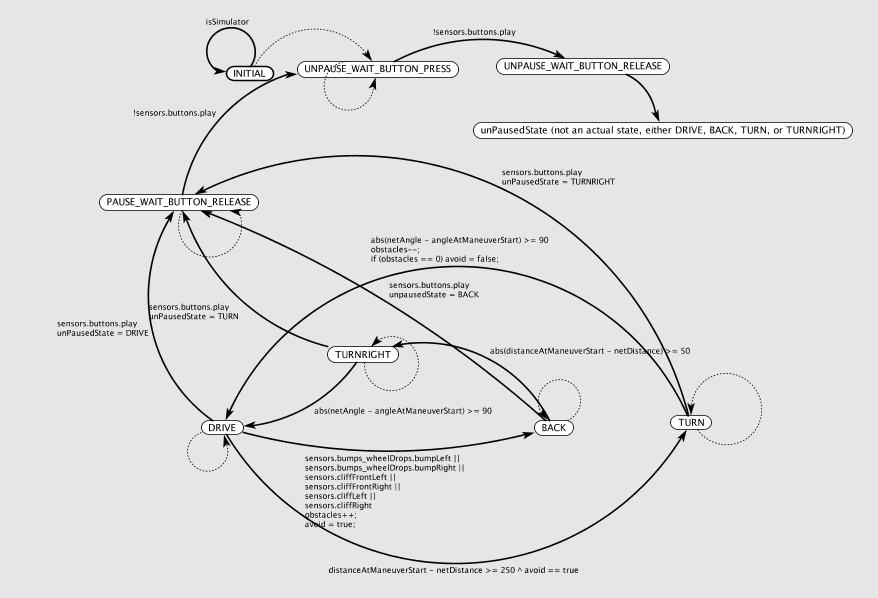
\includegraphics[width=1\textwidth]{../lab4_data/FSMLab4v2}
      \caption{Obstacle/Cliff avoidance FSM implemented in Lab 4}
    \end{figure}

  \section{Conclusion}
    Designing an obstacle/cliff avoidance algorithm was quite fun and rewarding when it actually worked. This was a very applicable problem for state machines and we can apply this technique to future problems that are similar in nature. This lab also helped us think about solving very simple human problems (avoiding an obstacle) step by step so that it can be applied to a robot.
\end{document}
